\documentclass[11pt, oneside, a4paper, titlepage]{article}
\usepackage[T1]{fontenc}
\usepackage[ttdefault=true]{AnonymousPro}
\usepackage[most]{tcolorbox} %For Formatting
\renewcommand*\familydefault{\ttdefault}
\usepackage[a4paper, portrait, margin=0.5cm]{geometry} %to make exact margins
\usepackage{tikz}
\usetikzlibrary{backgrounds}
\usepackage{fontawesome5}
\usepackage{graphbox}
\usepackage{accsupp}
\usepackage{trimclip}
\usepackage{xcolor}
\usepackage{sectsty}
\usepackage[compact]{titlesec}
\usepackage{ifthen}
\usepackage{calc} 
\usepackage{hyperref}

\titlespacing{\section}{0pt}{0pt}{0pt}
\AtBeginDocument{%                     
  \setlength\abovedisplayskip{0pt}
  \setlength\belowdisplayskip{0pt}}

\colorlet{body}{black!80!white}
\color{gray}

\newcommand{\itemmarker}{{\small\textbullet}}
\newcommand{\ratingmarker}{\faCircle}

\definecolor{Background}{HTML}{F5F5F5}
\definecolor{Highlight}{HTML}{78866B}

\sectionfont{\color{Highlight}}

\begin{document}

%Header Box

\tcbset{opacityback=0.7,enhanced jigsaw,colframe=Highlight,colback=Background, arc=5mm}
\begin{tcolorbox}
	\begin{minipage}{5cm} %Using Minipages to create two columns
		\hspace*{0.1cm}
		\begin{tikzpicture}
				\node[circle,
   				draw=gray,
   				text=white,
   				minimum size=4.25cm,
   				fill=Highlight] (c) at (0,0){Circle};
			\clip (0,0) circle(2cm);
			\node[anchor=center] at (0,-0.6) {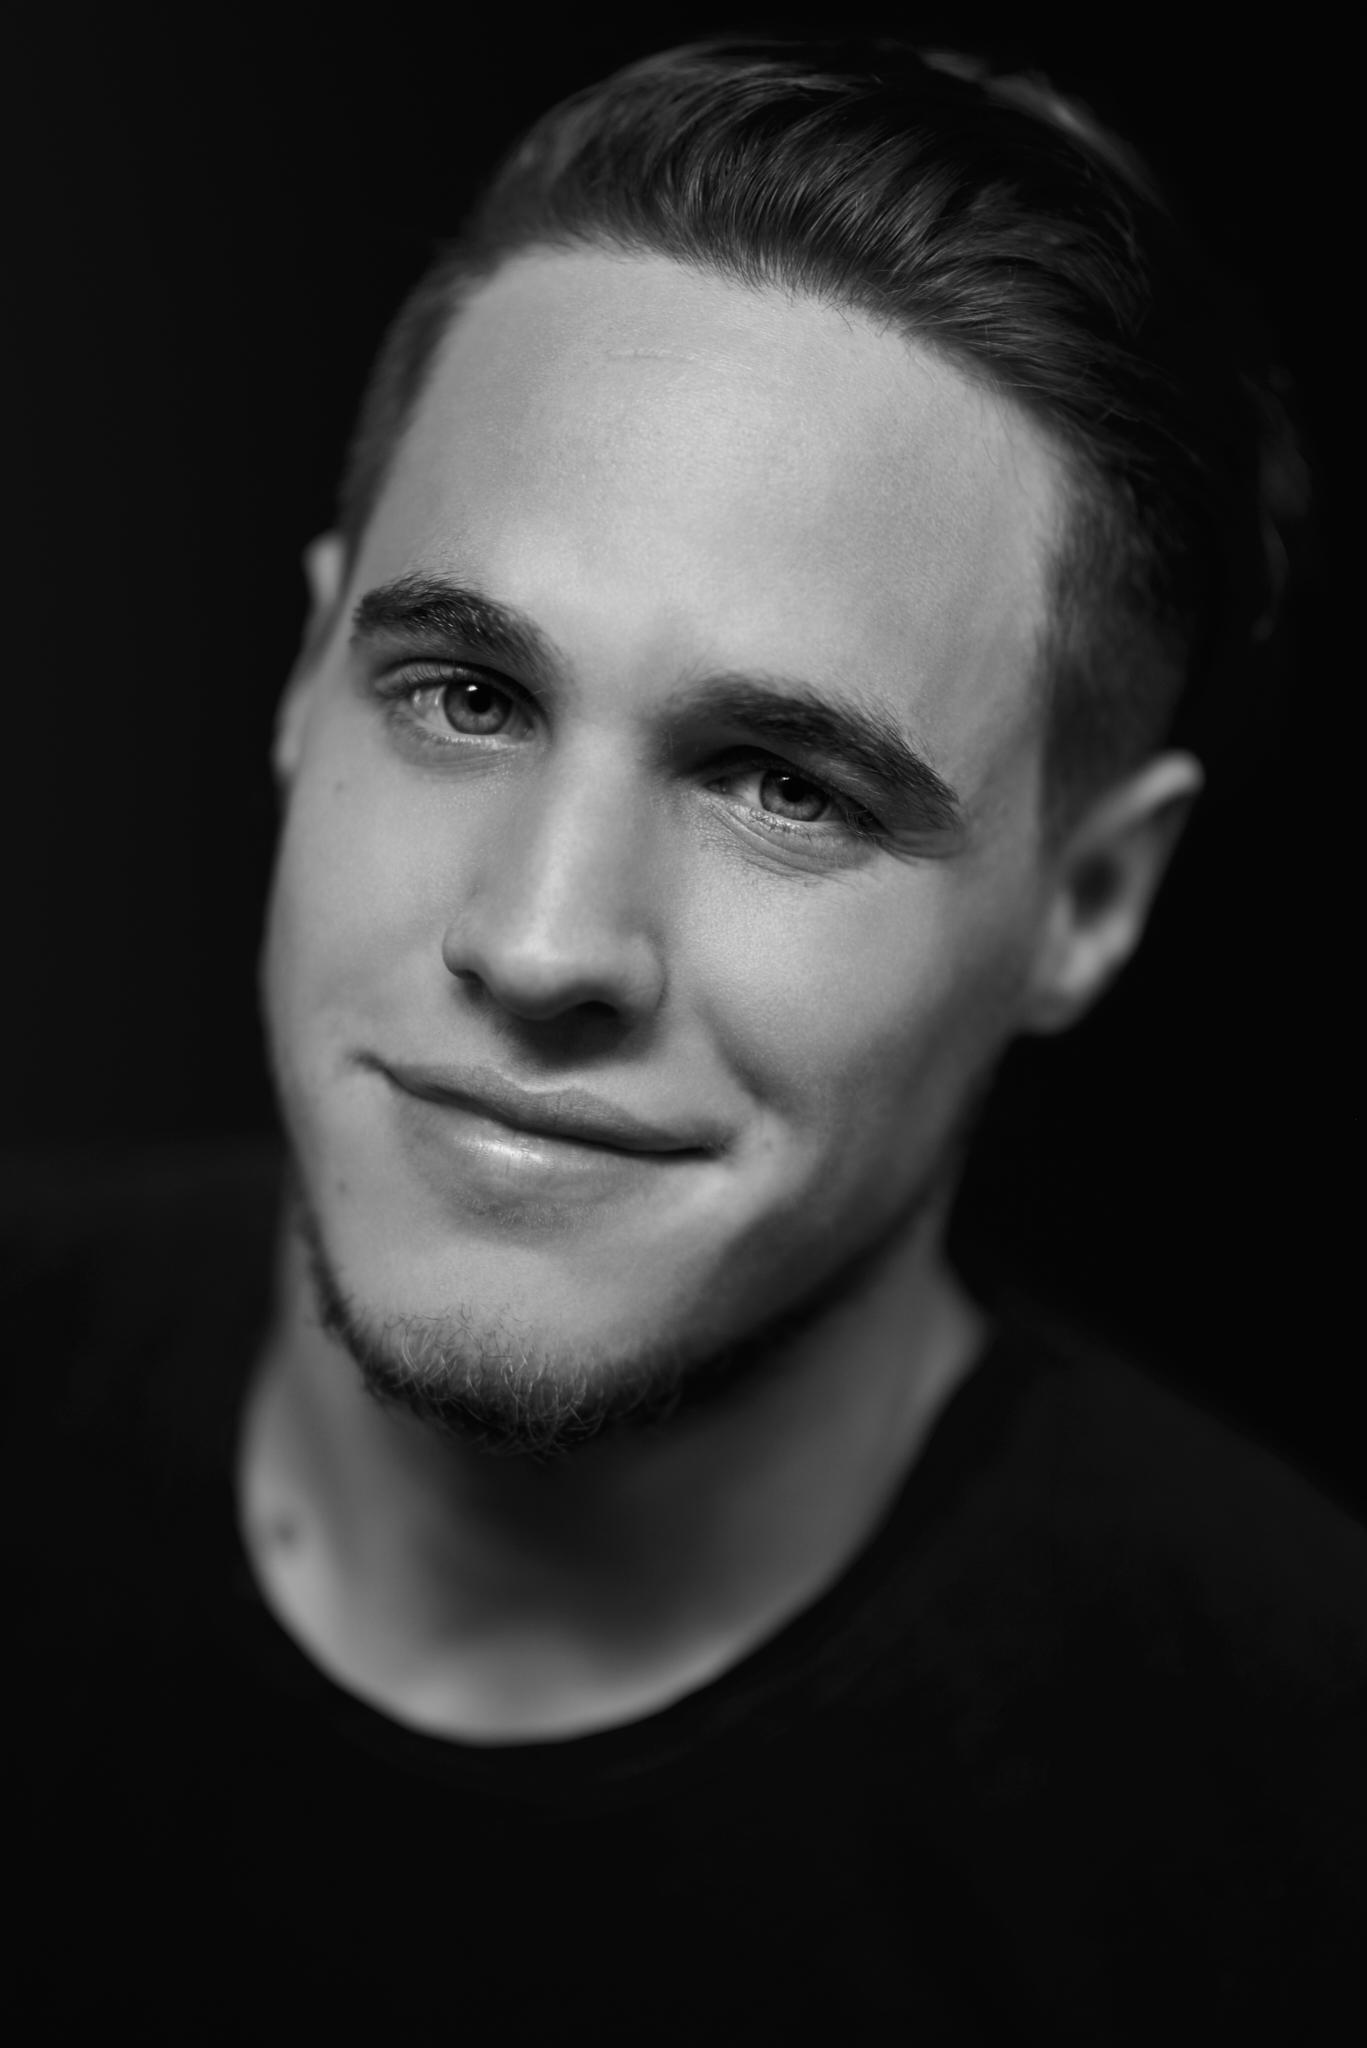
\includegraphics[width=4cm]{pic.jpg}};
		\end{tikzpicture}
	\end{minipage}
	\begin{minipage}{15cm}
		\begin{center}
			\Huge{\textcolor{Highlight}{Alejandro Garcia Sainz Sours}}
			\vspace*{0.5cm} 
			
			\huge{\textcolor{gray}{\emph{Software Developer}}}
		\end{center}
	\end{minipage}
\end{tcolorbox}

%Content 

\tcbset{colframe=white, colback=white, arc=10mm}
\newcommand\measurepage{\dimexpr\pagegoal-\pagetotal-\baselineskip\relax}

\begin{tcolorbox}[height fill]
	\begin{minipage}[t]{8cm}
		\vspace*{-0.25cm}
		\begin{tcolorbox}[grow to left by=0.6cm,opacityback=0.7, enhanced jigsaw, colback=Background, colframe=Highlight, arc=5mm]
		
			\section*{Profile \faIcon{male}}
			
			\begin{tabular}{r l}
				\textcolor{Highlight}{\faIcon{birthday-cake}} & April 9, 1994 \\
				\textcolor{Highlight}{\faIcon{flag}} & Mexico 
				
			\end{tabular}
			
			\section*{Contact \faIcon{paper-plane}}
			
			\large{
			\begin{tabular}{r l}
				\textcolor{Highlight}{\faIcon{mobile-alt}} & (55) 4581-4873 \\		
				\textcolor{Highlight}{\faIcon{github}} & \href{https://www.linkedin.com/in/aldpal/}{ALDPAL} \\					
				\textcolor{Highlight}{\faIcon{envelope}} & alexgss94@gmail.com \\		
				\textcolor{Highlight}{\faIcon{linkedin}} & \href{https://github.com/ALDPAL}{ALDPAL} 
			\end{tabular}}
			
			\section*{Technologies \faIcon{desktop}}
				\newcommand{\cvtag}[1]{%
					\tikz[baseline]\node[anchor=base,draw=Highlight,rounded corners,inner xsep=1ex,inner ysep =1ex,text height=1.5ex,text depth=.25ex]{#1};
					\hspace{-2ex}
					\vspace{0ex}
				}
				
					 \cvtag{Office}					
					 \cvtag{Unity}					
					 \cvtag{Monogame}
					 \cvtag{SDL}	
					 \cvtag{Openframeworks}
					 \cvtag{Processing}				
					 \cvtag{OpenGL}
					 \cvtag{DirectX 11}
					 \cvtag{Vulkan}
					 \cvtag{Arduino}
					 \cvtag{MySQL}
					 \cvtag{Git}
					 \cvtag{LaTeX}
					 \cvtag{Maya}
					 \cvtag{Blender}
					 \cvtag{Photoshop}
					 \cvtag{Premiere}
					 \cvtag{Illustrator}
					 \cvtag{Linux}
					 \cvtag{After Effects}					
					 \cvtag{Windows}
					 \cvtag{MacOS}
					 
			\section*{Languages \faIcon{language}}
				\graphicspath{{Flags/}}
				\newcommand{\flag}[1]{\includegraphics[align=c, width=1em]{#1}}
				\begin{tabular}{r l r l}
					\flag{MX.png} & Spanish & Level: & Native \\
					\flag{UK.png} & English & Level: & Native 	
				\end{tabular}								
				
			\section*{Programming \faIcon{code}}
			
				\newcommand{\cvskill}[2]{%
					\textcolor{black}{\textbf{#1}}\hfill
					\BeginAccSupp{method=plain,ActualText={#2}}
					\foreach \x in {1,...,5}{%
						\ifdimequal{\x pt - #2 pt}{0.5pt}%
						{\clipbox*{0pt -0.25ex {.5\width} {\totalheight}}{\color{Highlight}\ratingmarker}%
						\clipbox*{{.5\width} -0.25ex {\width} {\totalheight}}{\color{body!30}\ratingmarker}}
						{\ifdimgreater{\x bp}{#2 bp}{\color{body!30}}{\color{Highlight}}\ratingmarker}%
					}\EndAccSupp{}\par%
				}		
						
				\cvskill{C++}{3.5}
				\cvskill{C\#}{3.5}
				\cvskill{Python}{3}
				\cvskill{Java}{2.5}
				\cvskill{C}{2}		
				
			\section*{Soft Skills \faIcon{cloud}}		
				
				\cvskill{Critical Thinking}{5}
				\cvskill{Positive Attitude}{5}
				\cvskill{Work Ethic}{5}
				\cvskill{Leadership}{4}
				\cvskill{Teamwork}{3.5}
				\cvskill{Communicating}{3.5}
				
			\section*{Interest \faIcon[regular]{eye}}	
			
				\cvtag{Animals}
				\cvtag{Video Games}
				\cvtag{UFC}
				\cvtag{Crossfit}
				\cvtag{Ethical Hacking}
				\cvtag{Computer Graphics}
				\cvtag{Anime}
				\cvtag{Crypto}								
			
			\vspace*{0.1cm}
				
		\end{tcolorbox}
	\end{minipage}	
	\begin{minipage}[t]{11cm}
	
		\vspace*{-0.25cm}
		
		\begin{tcolorbox}[opacityback=0.7, enhanced jigsaw, grow to right by=0.2cm, colframe=Highlight, colback=Background, arc=5mm]
			
			\newcommand*{\cvsection}[1]{\section*{#1}}
				\titleformat{\section}%
					{\color{Highlight}\normalfont\bfseries\LARGE}{}{0pt}{}
				\titlespacing*{\section}{0pt}{0pt}{-10pt}
			
			\setlength{\tabcolsep}{0pt}

			\newenvironment{cvtable}[1][1]{%
				\renewcommand{\arraystretch}{#1}%
				\begin{tabular*}{\textwidth}{@{\extracolsep{\fill}}ll}%
			}{%
				\end{tabular*}%
			}		
			
			\newcommand{\cvitem}[4]{%
				\parbox[t]{0.15\textwidth}{\raggedright #1} &%
				\parbox[t]{0.90\textwidth}{%
					\if\relax\detokenize{#4}\relax%
						\parbox[t]{\linewidth-\widthof{\footnotesize #3}-1em}{\raggedright #2}%
					\hfill {\footnotesize#3}%
					\else%
						\parbox{\linewidth-\widthof{\footnotesize #3}-1em}{%
							\raggedright \textbf{#2}%
						} \hfill {\footnotesize#3} \\%
						\textcolor{black}{#4} \vspace{\parsep}
					\fi%
				}\\
			}		
			
			\cvsection{Education \faIcon{university}}
			\begin{cvtable}[3]
				\cvitem{2017 -- 2020}{Video Game Programming}{SAE Institute México}{Thesis:Compilation of Development Resources and Ray Tracing with Vulkan}
			\end{cvtable}	
			
			\cvsection{Certificates \faIcon{certificate}}
				\begin{cvtable}[3]
					\cvitem{2021}{Introduction to Cybersecurity}{CISCO}{ }
				\end{cvtable}		
				
			\cvsection{Employment History \faIcon{handshake}}
			\begin{cvtable}[3]
				\cvitem{2014 -- 2015}{Assistant}{Mauricio Garcia Sainz}{Financial document analysis for proper distribution and filing purposes. Assisted with operational activities. Developed a procedure for market investigation, evaluation and registration.}
			\end{cvtable}
			
			\cvsection{Social Service \faIcon{hands-helping}}
			\begin{cvtable}[3]
				\cvitem{2017}{Volunteer}{Un Techo Para Mi País}{Taught English lessons to children and adults from humble socioeconomic backgrounds. Took part in a massive survey research targeted at households living in extremely humble conditions.}
				\cvitem{2020 -- 2021}{Volunteer}{Medusa Lab}{Utilized Kinect V1 to track user gestures and leverage its body tracking functionality on Unity (specifically on VFX Graph). Particle systems were mapped to a 3D model or 2D texture. Additional features included particle transitions and reaction to the audio spectrum of an audio file. This was used to compose an audiovisual experience for a specific piece of music.}
			\end{cvtable}			
		\end{tcolorbox}
	\end{minipage}	
\end{tcolorbox}
\end{document}




